\documentclass{article}
\usepackage[utf8]{inputenc}
\usepackage{algorithm}
\usepackage{algpseudocode}
\usepackage{graphicx}
\usepackage{wrapfig}
\usepackage{geometry}
 \geometry{
 a4paper,
 total={170mm,257mm},
 left=20mm,
 top=20mm,
 }
\title{Drug Consumption: A Machine Learning Analysis of Marijuana 
and Other Drug Users}
\author{Priyanshi Aeron, Samantha Anthony, Zachary Hudgins, Tarini Ramesh}
\date{}

\begin{document}

\maketitle
\vspace*{-8mm}
\section{Introduction}
\vspace*{-2mm}
According to the United States Centers for Disease Control and Prevention (CDC), there is a drug epidemic in the U.S. The number of drug overdose deaths has quadrupled from 1999 to 2019, and the recent COVID-19 pandemic has only exacerbated these issues and increased deaths. Considering the alarming rate of this trend, it is imperative to find the causes of fatal drug use in order to save lives and reverse the negative impact on communities and the economy ({\it Understanding the Epidemic}).
Many reports over the years have suggested that marijuana use leads to the use of other illicit substances, typically those with more harmful effects. However, marijuana has recently become more popular and prevalent, as more than half of the states in the U.S. have legalized, at the very least, the medical use of it. As more states work to legalize it, and as activists work to legalize it at a federal level, it is of the utmost importance to understand whether cannabis leads to using other illicit substances, and thus to fatal overdosing. In this paper, we explore if cannabis usage correlates with the usage of other illicit substances.


\vspace*{-4mm}
\section{Literature Review}
\vspace*{-2mm}
The Drug and Alcohol Dependence Journal: An International Journal on Biomedical and Psychosocial Approaches published an article on evaluating the “gateway” drug theory. Researchers investigated the gateway drug theory by looking at the risk of later drug use in one’s life conditional on the use of drugs earlier in one’s life. They compared various gateway drugs, such as alcohol, tobacco, and cannabis, to other illicit drug use, such as cocaine, opium, and heroin across 17 countries. For the most part, the study concluded that substances used earlier in one’s life predicted higher drug use later in one’s life. However, these associations differed from country to country. For instance, the use of marijuana was more strongly associated with later illicit drug use in the US, Spain and Belgium, than it was in the Netherlands. Typically, cannabis is most often the first illicit drug used, and it is generally preceded by tobacco and alcohol use (Degenhardt, L. et al., 2010).  
According to the National Institute on Drug Abuse, a study using longitudinal data found that those who used marijuana were more likely to develop an alcohol use disorder within 3 years, compared to those who did not use marijuana. The NIDA also found that early exposure to cannabinoids leads to decreased reactivity of brain dopamine centers later in life, thus supporting the pre-existing notion that marijuana is a gateway drug. However, it is important to note they found that the majority of people do not go onto using more harmful drugs ({\it Is marijuana a gateway drug?}).

There is also epidemiologic evidence that young marijuana smokers are much more likely than non-smokers to try hallucinogens, per research from the Johns Hopkins Bloomberg School of Public Health. The researchers gathered data from 40,000 people. They found those who used marijuana had more opportunity to use other hallucinogens, and even when users and non-users of marijuana were presented with the same opportunity to use other hallucinogens, users of marijuana were more likely to use the other drugs. The researchers suggest that a large difference between those who use marijuana versus those who do not are social influences. Developing contact with illegal drug dealers for marijuana could lead them to being pushed to trying other illegal substances such as LSD or ecstasy, thus creating a correlation between marijuana and those types of drugs ({\it Marijuana use linked to hallucinogen use: Johns Hopkins}).	
A study by the Frontiers of Neuroscience delved into drug disorders and the concurrent use of drugs such as alcohol, opioids, and heroin. The study aimed to highlight potential methods to move forward with the task of examining polysubstance disorders so individuals can be treated accordingly. Researchers found that 11.3\% of individuals that are diagnosed with a substance use disorder have concurrent alcohol and illicit use disorders. This shows that the use of a drug can lead to the increased use of other drugs. They also reported that the increased risk of developing heroin dependence is twofold for alcohol misusers, threefold for marijuana users, 15 fold for cocaine users, and 40 fold for prescription misusers. This study helps prove the correlation between different drug users. Additionally, they found that the significant use of nicotine in younger age groups led to increased chances of marijuana misuse as they grew older. Overall, the study concluded that polysubstance abuse is a widespread problem that is not being tackled at the root (Crummy et al., 2020). 
 

\vspace*{-4mm}
\section{Study Data}
\vspace*{-2mm}
Our data was pulled from the University of California - Irvine Machine Learning Repository. This repository consists of 622 datasets that can be used by the machine learning community. Our multivariate data set on drugs was donated to the archive in 2016 by four researchers from the UK. It consists of 1885 respondents and 32 attributes. Respondents were classified based on 12 main attributes such as age, location, and personality measurements and were questioned about 18 legal and illegal drugs and one fictitious drug. Some of the real drugs include nicotine, marijuana, and mushrooms and the fake drug was called “Semeron.” Respondents were told to place the drugs into seven classes such as "Never Used", "Used in Last Year", and "Used in Last Day". All attributes in the dataset were originally categorial and they were quantified. Although this is useful in many cases it was difficult to understand the different attributes and the dataset with purely numerical values, so our first step in cleaning the dataset consisted of converting the quantified attributes back to categorical ones. The next step of cleaning the data involved removing the fictitious drug and the respondents who “used” this drug. We want our dataset to be practical and applicable in the real world and future studies so we decided to drop the fake drug and respondents who lied about using it. After that, we decided to group the respondents and drugs to better identify trends and categorize the data. We grouped the respondents by classifying them as users and non-users. Respondents that reported that they have "Never Used" a drug were labeled as non-users and all other answers classified the respondents as users. This made the data binary and allowed for more accurate models. Another way we grouped the data was by drug scheduling according to the US Drug Enforcement Administration. An important attribute to note about our dataset is that it includes respondents from all over the world, however, we used the US DEA drug scheduling as a basis for grouping the drugs ({\it Drug scheduling}). Overall, cleaning the data allowed for a much easier understanding of the dataset and for a smoother creation process of the models.  
\vspace*{-4mm}
\section{Methodology}
\vspace*{-2mm}
In order to investigate our question of marijuana use as it relates to other drug use, we generated and tuned many different models to predict the ‘usage of cannabis’ classification of a given participant. We modeled logistic classification, support vector machine, random forest, and a neural network due to their prominence and historic aptitude for binary classification tasks.
\vspace*{-4mm}
\subsection{Logistic Classification}
\vspace*{-2mm}
The first model we generated was logistic regression. Logistic regression is a relatively simple model that generates the probability of a discrete outcome given an input variable. For binary classification, we had our independent variables be all drugs except cannabis, while the dependent was cannabis. We did a 80/10/10 train/validation/test split and with logistic regression got a 0.888 accuracy score. 
\vspace*{-4mm}
\subsection{Support Vector Machine}
\vspace*{-2mm}
\begin{wrapfigure}{r}{6cm}
  \centering
  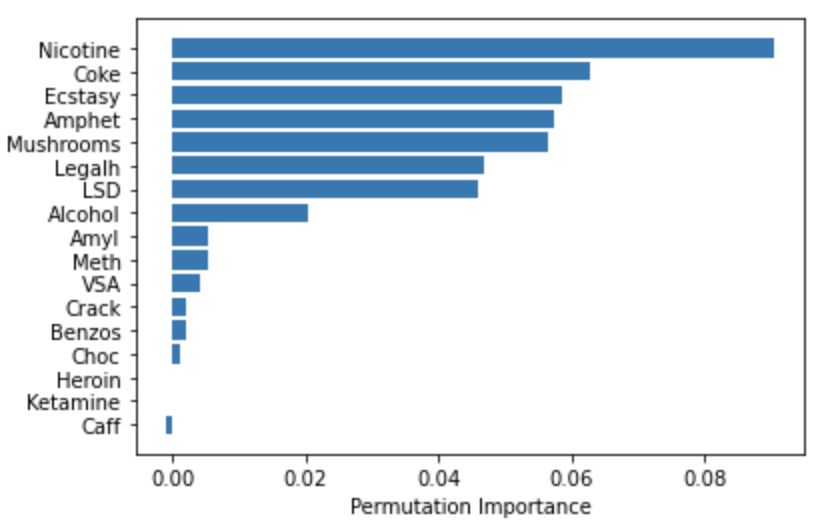
\includegraphics[height=4cm]{Feature.png}
\end{wrapfigure}
Another model we used was a support vector machine. Support vector machines (SVMs) are a set of supervised methods used mainly for classification and regression. They are high speed machine learning models that perform well even with a limited number of samples. In order to create an SVM, we had to do a 80/10/10 train/validation/test split on our data. For the first SVM, we created a multiclass model. The accuracy of this model came out to 0.457. In order to increase the accuracy of the model, we decided to switch to a binary SVM by making “never used” the drug one group and all the other answers that involved any use of the drug as the other group. We ran the model again and this time it resulted in 0.867 accuracy. For the first two models the kernel was set to linear. To explore more models and in an attempt to increase the accuracy of the model even more we tried to explore with other kernels. We decided to run the gaussian (rbf) and sigmoid kernels. The sigmoid kernel accuracy came out to 0.878, an improvement from the previous. The Gaussian kernel accuracy came out to 0.894, making it the best SVM model generated. The linear model, as the name suggests, only allows for divisions between the classes by linear lines. The other models allow for curves and other shapes to create the division between the classes. The latter models allowed for more room for the model to adjust to the data, and therefore, led to higher accuracy scores. In order to gain a deeper understanding of the data from the best SVM, we decided to create a feature importance graph. According to the graph, the top five determining factors of whether or not a participant was a marijuana user was if they used nicotine, coke, ecstasy, amphetamines, and mushrooms.
\vspace*{-4mm}
\subsection{Random Forest}
\vspace*{-2mm}
The next model generated was a Random Forest model. A Random Forest is a powerful classifier that uses an ensemble of relatively uncorrelated decision trees which are then used as a whole to vote on which class each data point belongs to. To begin, we started from the bottom by building a single decision tree to get a baseline of how much our base model could stand to improve. This resulted in a base model accuracy of 0.848 and an AUC, or area under the receiver operating characteristic (ROC) curve, of 0.795. Next, we generated a base model for a random forest, which resulted in an accuracy of 0.8963 and AUC of 0.948. Since an AUC of 1.0 means perfect classification, and the random forest’s AUC was higher, it was easy to conclude that the random forest was better than just the single decision tree. However, even with these strong accuracy and AUC measurements, the random forest could be improved by some parameter tuning. To tune the hyperparameters, the metric we aimed to minimize was the out-of-bag (OOB) error, a standard measure of prediction error for random forests using bootstrapping, which averages prediction error on observations not used to generate the next tree. The hyperparameters that were tuned were the splitting criteria for each node, number of features for best split, maximum depth of the individual trees, and number of decision trees in the forest. Various values for each of these hyperparameters were tested against different random forests of many sizes. This hyperparameter tuning is displayed in the graphs and interpreted below.

\begin{figure}[htp]
    \centering
    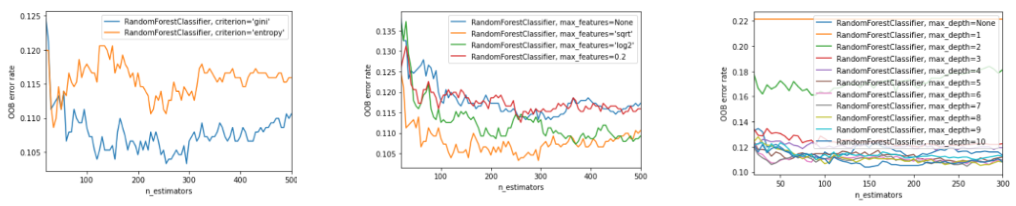
\includegraphics[width=12cm]{RF_hyperparameter_tuning.png}
    \label{fig:randforest}
\end{figure}
\vspace*{-4mm}

From the first graph, we can conclude that gini is the better criterion to minimize OOB error at larger values of the number of estimators used for the random forests. Additionally, the optimal maximum features parameter is the square root because it stabilizes to the lowest OOB error at the larger numbers of estimators. From the final graph, the maximum tree depths above around four all begin to converge to a very small OOB error, therefore the default parameter of no max depth was chosen because it produced the same results as the other depths. Finally, all of these values converged to low OOB errors around 150 to 300 decision trees, or estimators, in the forest, so the number of 250 decision trees was chosen due to it being in the range and not drastically increasing model computation time. After all the hyperparameter tuning, the model generated resulted in an accuracy of 0.915 and an AUC of 0.955. Therefore, the new tuned model was more accurate and had a larger AUC than the base models before, meaning it was a better model for the data.
\vspace*{-4mm}
\subsection{Neural Network}
\vspace*{-2mm}
The final type of model trained on the dataset were neural networks. This model is one method of deep learning, where the model is able to create a large number of non-linear relations between input features. It is then able to re-categorize the input features into new, learned features that can be stronger estimators of the target data. This is due to its hidden layers of nodes that act as inputs to the next hidden or output layer, which each get their weights and biases tuned via backward propagation while training. This model was trained both as a multiclass and binary classifier in our scenario. The results of the multiclass classifier were quite poor, topping out at around 28\%. However, due to the nature of the target output always having exactly one class chosen, the final prediction of the model was changed to be determined by the single output node with the highest probability, which upped the prediction accuracy to 45.2\%. This fixed the issue where the multiclass classifier would sometimes predict no class at all or multiple classes. However, as seen in the confusion matrices, the vast majority of the predictions were of only 2 out of 7 possible classifications, so the final model was not as robust as hoped for. When trained for binary classification, the model performed much better, reaching a 91.5\% prediction accuracy. Each model had its hidden layer setup chosen by testing on models with $2^{n}$ nodes, for n inclusive between n and 6, for each of both 1 and 2 hidden layers, and selecting the best performing arrangement. This range was chosen primarily regarding the trainings done with only data of the 17 other drugs, so having a top end of 64 nodes is a reasonable expectation for new connections between the data to be formed. Furthermore, the dataset is not complex or expansive enough to warrant more than 2 hidden layers, which can find the majority of non-linear relationships and new features that deep learning seeks to accomplish. Each additional layer also greatly increases the cost of computation to train, so a smaller domain is preferable.
\vspace*{-4mm}
\section{Results}
\begin{wrapfigure}{r}{6cm}
  \centering
  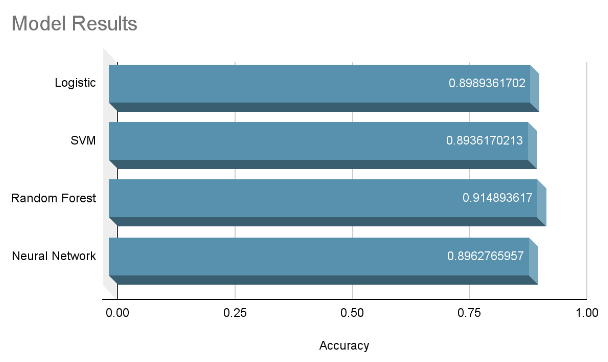
\includegraphics[height=4cm]{model_results.png}
\end{wrapfigure}
\vspace*{-2mm}
The models generated to answer our question were all decent models, as described above. They were all able to predict labels on the test set fairly well. As evident in the Model Results figure, the model that produced the most accurate classification was the Random Forest. It is worth noting that all the models had around 90\% accuracy and similarly high precision. However, due to its higher accuracy and in-depth analysis features, the Random Forest model was chosen as our best model to solve this task. After testing the optimized model, the random forest resulted in an AUC of 0.955 and an accuracy of 0.915 on the test set. The ROC curve, confusion matrix, and algorithm are displayed above, in order. Following the creation and verification of that model, we started looking into how the random forest was able to conclude who was a marijuana user and who had never used it. To do so, we looked at feature importance.
\begin{figure}[htp]
\centering
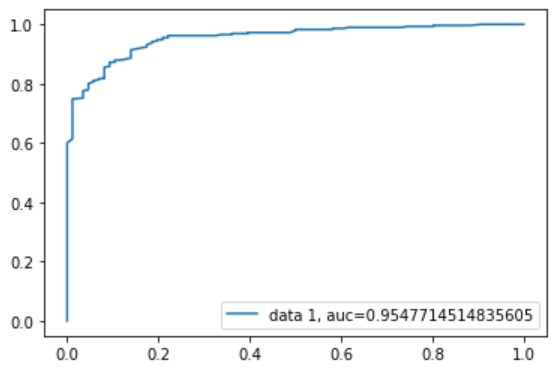
\includegraphics[width=.2\textwidth]{rf_auc_curve.png}\hfill
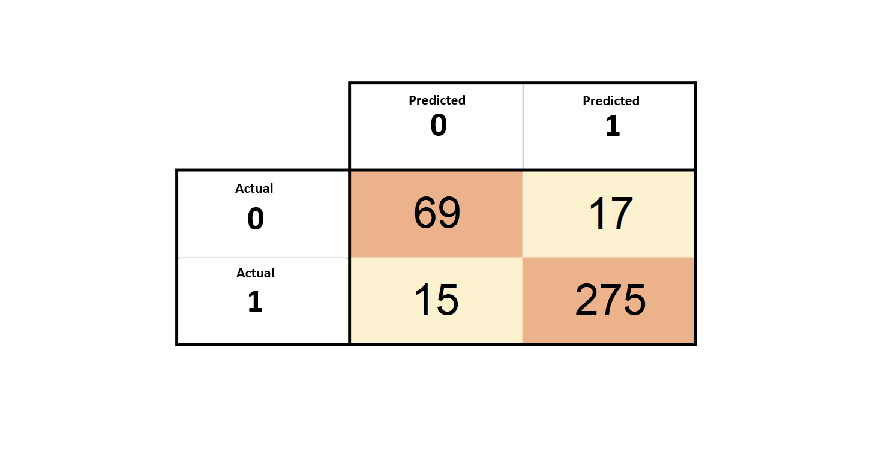
\includegraphics[width=.2\textwidth]{rf_conf_matrix.png}\hfill
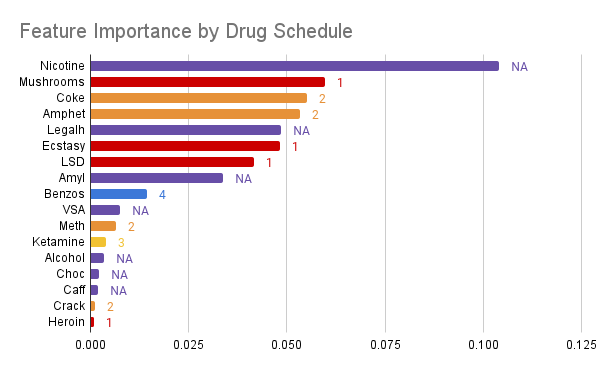
\includegraphics[width=.3\textwidth]{Feature Importance by Drug Schedule.png}\hfill
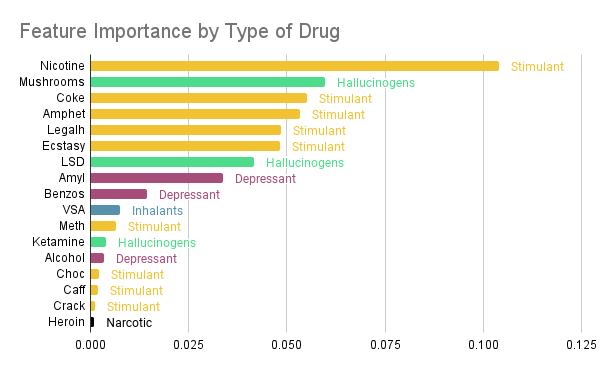
\includegraphics[width=.3\textwidth]{Feature Importance by Type of Drug.png}
\end{figure}

According to the model, the most important determining factor of whether or not a participant was a marijuana user was if they used nicotine. This aligns with previously conducted research on marijuana users and nicotine smokers. This relationship could be due to the fact that these drugs are easily accessible, however other easily accessible drugs like alcohol or caffeine were not important features. Therefore, there is something about nicotine that is specifically correlated to marijuana use, such as the documented interactive effects. Next, we colored the feature importances according to which schedule the drug is, as determined by the United States Drug Enforcement Administration ({\it Drug Scheduling}). As you can see in the chart above, marijuana (schedule 1) did not simply lead to other schedule 1 or 2 drugs as a whole. In fact, heroin, a major schedule 1 drug, and meth, a major schedule 2 drug, are not significantly related to marijuana use, according to the model. Some of the primary features that help predict marijuana use are actually unscheduled. Therefore, one cannot conclude that marijuana use will automatically lead to using major schedule 1 drugs as a whole. Finally, we looked into the types of drugs that were correlated with marijuana use in the above graph on the right ({\it Drugs of Abuse - Uses and Risks}). Marijuana is a hallucinogen and stimulant, resulting in the hypothesis that weed use would lead to similar drug use. This hypothesis is supported by the figure which shows a high correlation between marijuana use and other hallucinogens and stimulants, such as nicotine, mushrooms, and cocaine. Instead of leading to depressants or narcotics, marijuana use was primarily correlated to users of similar hallucinogenic and stimulant drugs.
\vspace*{-4mm}
\section{Future Research}
\vspace*{-2mm}
One goal that was missed out on within the scope of this project was a strong ability to predict which frequency of cannabis use class a user fell under, rather than simply user or not user. Additionally, it is not exceptionally clear why these multiclass models failed to do so because some of the most prevalent models learn their own features out of the provided data. Thus the aggregated weights and biases do not make it clear which originally input features create strong or weak correlation with a certain output classification. With more time or in a future study with stronger model measuring tools, a more in-depth analysis of the trained multiclass models could provide readings of what the models were using to predict the timeframe of usage. This would enable a more robust insight into indicating if cannabis is used alongside certain other drugs concurrently, if cannabis is replaced by specific other drugs and thus acts as a gateway, or if cannabis is used as replacement for specific drugs.
\vspace*{-4mm}
\section{Conclusion}
\vspace*{-2mm}
Our analysis provided worthwhile findings intrinsically, confirmed existing notions found in other literature, and posed challenges to overcome in similar future studies. Firstly, due to the high accuracy of the binary classification models and the strong feature importance of drugs such as mushrooms, cocaine, and especially nicotine on these predictions, it is clear that cannabis use is strongly connected to the usage of at least certain other drugs. This does give some accreditation to the thought of cannabis being a gateway drug. However, our findings also showed a rather low connection to drugs such as heroin, crack, and alcohol, which respectively correspond to the same schedulings as the 3 previously mentioned indicative drugs. Therefore, it is certainly not enough to describe cannabis as a gateway drug in a definitive, all-encapsulating manner. 
Our findings did also show all the hallucinogens, such as mushrooms, LSD, and ecstasy, near the top of the greatest feature importance and none near the bottom. This supports the specific claims of cannabis use being associated with other hallucinogens, and is apparent as the connection to all other hallucinogens measured in the study is quite strong, which is not true for other categories of drugs.



\section{Works Cited}
\begin{itemize}
\setlength{\emergencystretch}{3em}
\item Crummy, E. A., O’Neal, T. J., Baskin, B. M., \& Ferguson, S. M. (2020, June 16). One is Not Enough: Understanding and Modeling Polysubstance Use. Frontiers, https://www.frontiersin.org/articles/10.3389/fnins .2020.00569/full

\item Drug scheduling. DEA. (n.d.). Retrieved from https://www.dea.gov/drug-information/drug-scheduling 

\item Drugs of Abuse - Uses and Risks. Oregon State University Human Resources. (2019, July 12). Retrieved from https://hr.oregonstate.edu/employees/current-employees/health-wellness-and-safety/drug-free-workplace/drugs-abuse-uses-and 

\item Degenhardt, L. et al. (2010, April). Drug and Alcohol Dependence. Science Direct. Retrieved from https://www-sciencedirect-com.libproxy.lib.unc.edu/science/article/pii/S0376871609004219?via=ihub 

\item Is marijuana a gateway drug? National Institutes of Health. (2021, May 24). Retrieved from https://nida.nih.gov/publications/research-reports/marijuana/marijuana-gateway-drug 

\item Marijuana use linked to hallucinogen use: Johns Hopkins. Johns Hopkins Bloomberg School of Public Health. (n.d.). Retrieved from https://publichealth.jhu.edu/2002/marijuana-hallucinogen 

\item Understanding the epidemic. Centers for Disease Control and Prevention. (2021, March 17). Retrieved from https://www.cdc.gov/drugoverdose/epidemic/index.html 
\end{itemize}

\end{document}
